% !TeX root = ../../Book1.tex
% 纲要标题：### 7.2 曲线基本定理
% 纲要位置：几何学计划纲要.md，第 376 行。
% 正文状态：初稿；尚未正式审核。

% 纲要内容开始
% 
% * 标架常微分方程的存在与正交性保持
% * 从标架积分得到曲线
% * 刚性变换意义下的唯一性
% * 给定不变量与曲线闭合的额外条件
% 
% 纲要内容结束

\section{曲线基本定理}
\label{g1:sec:0702}

曲率与挠率是从曲线求导得到的两个函数。反过来，若只知道每一点弯曲多少、密切平面如何转动，能否恢复曲线？Frenet 方程提供了一种办法：先恢复三个随动的单位向量，再把切向量积分成位置。这里有两个需要分别回答的问题：方程是否有解，解出来的三个向量是否始终构成正交标架。Frenet 方程的斜对称系数将使内积导数为零，把初值处的正交性传到整个区间。

\subsection{标架常微分方程的存在与正交性保持}
\label{g1:subsec:0702:01}

下面以连续函数的积分、函数级数的一致收敛和微积分基本定理证明所需的线性常微分方程结论。以下区间均有非空内部；在区间包含的端点处，导数按单侧理解。

\begin{lemma}[连续系数线性方程]
	\label{g1:lem:linear-frame-ode}
	设 \(I\subseteq\mathbb R\) 是具有非空内部的区间，\(s_0\in I\)，\(A\colon I\rightarrow M_m(\mathbb R)\) 连续，端点处的导数按单侧理解。对任意 \(u_0\in\mathbb R^m\)，存在唯一的 \(C^1\) 函数 \(u\colon I\rightarrow\mathbb R^m\)，满足
	\[
		u'(s)=A(s)u(s),\qquad u(s_0)=u_0.
	\]
	特别地，连续矩阵系数方程 \(F'=FA\) 或 \(F'=AF\) 也有指定矩阵初值的唯一全区间解。
\end{lemma}

\begin{proof}
	把求导方程改写为积分方程
	\[
		u(s)=u_0+\int_{s_0}^s A(t)u(t)\,\mathrm{d}t.
	\]
	从常向量开始逐次积分，令
	\[
		u_0(s)=u_0,\qquad u_{j+1}(s)=\int_{s_0}^s A(t)u_j(t)\,\mathrm{d}t.
	\]
	这里 \(u_j\) 是将要相加的第 \(j\) 项，而不是第 \(j\) 次近似解。取包含 \(s_0\) 的任意紧子区间 \(J\subseteq I\)，令 \(M=\max_{t\in J}\lVert A(t)\rVert\)，范数取 Euclid 范数诱导的算子范数。反复积分并归纳可得
	\[
		\lVert u_j(s)\rVert\leq\lVert u_0\rVert\frac{M^j|s-s_0|^j}{j!},\qquad s\in J.
	\]
	当 \(s<s_0\) 时将积分反向后取绝对值，同一估计仍成立。于是级数 \(u=\sum_{j=0}^{\infty}u_j\) 在 \(J\) 上一致收敛。系数 \(A\) 有界，故可以把求和移入积分，得到上面的积分方程；被积函数连续，微积分基本定理便给出 \(u\in C^1\) 及 \(u'=Au\)。

	为证唯一性，设两解之差为 \(w\)，则 \(w(s_0)=0\) 且 \(w(s)=\int_{s_0}^s A(t)w(t)\,\mathrm{d}t\)。记 \(K=\max_J\lVert w\rVert\)，反复代入同一积分式，任意 \(j\geq0\) 均有
	\[
		\lVert w(s)\rVert\leq K\frac{M^j|s-s_0|^j}{j!}.
	\]
	右端随 \(j\to\infty\) 趋于零，故 \(w=0\)。

	每个 \(s\in I\) 都与 \(s_0\) 同处某个这样的紧区间。上述积分项在所有区间上由同一公式定义，因此得到 \(I\) 上的同一个解；无需假定 \(I\) 有界，也不要求 \(A\) 在整个 \(I\) 上有统一上界。矩阵方程 \(F'=AF\) 对每一列应用已证结论；\(F'=FA\) 则先转置，再对每一列应用它。
\end{proof}

上述阶乘估计解释了线性方程为何不会在有限的内部参数值处突然失去解：只要系数在这一点附近连续，紧区间上的整串积分仍然收敛。端点若不属于 \(I\)，则可能出现发散。例如 \(u'=u/(1-s)\) 在 \(I=(-\infty,1)\) 上的解可能在 \(s\to1\) 时发散。

\ProseParagraphBreak

把右手正交标架写成以向量为列的矩阵 \(F=(T,N,B)\)。由\cref{g1:prop:frenet-equations}，我们要解的是
\begin{equation}
	\label{g1:eq:frenet-matrix}
	F'=FA,\qquad
	A(s)=
	\begin{pmatrix}
		0&-\kappa(s)&0\\
		\kappa(s)&0&-\tau(s)\\
		0&\tau(s)&0
	\end{pmatrix}.
\end{equation}
第一列说 \(T'=\kappa N\)，第二列说 \(N'=-\kappa T+\tau B\)，第三列说 \(B'=-\tau N\)。矩阵 \(A\) 的各列记录导向量在当前标架中的系数，因此乘法写在右边。

\ProseParagraphBreak

行列式为 \(1\) 的正交矩阵组成\term[teshuzhengjiaoqun]{特殊正交群}[special orthogonal group]，这里记
\[
	\operatorname{SO}(3)\coloneqq\{Q\in M_3(\mathbb R):Q^{\mathsf T}Q=I,\ \det Q=1\}.
\]
它的列向量正好是右手正交标架。\symidx{\(\operatorname{SO}(3)\)：三维特殊正交群}

\begin{proposition}[斜对称系数保持标架]
	\label{g1:prop:skew-frame-orthogonality}
	设 \(I\subseteq\mathbb R\) 为具有非空内部的区间，\(s_0\in I\)，\(A\colon I\rightarrow M_3(\mathbb R)\) 连续且 \(A^{\mathsf T}=-A\)。设 \(F:I\to M_3(\mathbb R)\) 是方程 \(F'=FA\) 的 \(C^1\) 解，端点导数按单侧理解。若其初值 \(F(s_0)\) 属于 \(\operatorname{SO}(3)\)，则 \(F(s)\in \operatorname{SO}(3)\) 对每个 \(s\in I\) 成立。
\end{proposition}

\begin{proof}
	\cref{g1:lem:linear-frame-ode}给出全区间的 \(C^1\) 解。直接求导可得
	\[
		(FF^{\mathsf T})'=FAF^{\mathsf T}+FA^{\mathsf T}F^{\mathsf T}=0.
	\]
	因此 \(FF^{\mathsf T}=I\)。这使 \(F\) 可逆，且 \(F^{-1}=F^{\mathsf T}\)，从而也有 \(F^{\mathsf T}F=I\)。正交矩阵的行列式只能为 \(1\) 或 \(-1\)；它随 \(s\) 连续，而区间连通，所以只能恒等于初值 \(1\)。
\end{proof}

斜对称性恰好使长度与内积的变化抵消，因而把初值的一次正交条件传播到整个区间。

\subsection{从标架积分得到曲线}
\label{g1:subsec:0702:02}

现在可以把“弯曲和扭转决定形状”写成精确结论。条件 \(\kappa>0\) 保证 \(N=T'/\kappa\) 有意义；正则性条件则保证所得曲线确实具有本章用三阶导数定义的经典挠率。

\begin{theorem}[空间曲线基本定理：存在性]
	\label{g1:thm:space-curve-fundamental}
	设 \(I\subseteq\mathbb R\) 为具有非空内部的区间，\(\kappa\in C^1(I)\) 处处为正，\(\tau\in C^0(I)\)，端点处的导数按单侧理解。给定 \(s_0\in I\)、点 \(p_0\in\mathbb R^3\) 和右手正交标架 \((T_0,N_0,B_0)\)，存在唯一的 \(C^3\) 单位速率曲线 \(\gamma\colon I\rightarrow\mathbb R^3\)，使其曲率、挠率分别为 \(\kappa,\tau\)，并满足
	\[
		\gamma(s_0)=p_0,\qquad
		(T,N,B)(s_0)=(T_0,N_0,B_0).
	\]
	这一结论称为\term[quxianjibendingli]{曲线基本定理}[fundamental theorem of space curves]。
\end{theorem}

\begin{proof}
	用给定的 \(\kappa,\tau\) 组成\eqref{g1:eq:frenet-matrix}中的连续斜对称矩阵，解出初值 \(F(s_0)=(T_0,N_0,B_0)\) 的方程。由\cref{g1:prop:skew-frame-orthogonality}，三个列向量始终是右手正交单位向量。定义
	\begin{equation}
		\label{g1:eq:curve-frame-integral}
		\gamma(s)=p_0+\int_{s_0}^s T(t)\,\mathrm{d}t.
	\end{equation}
	于是 \(\gamma'=T\)，速率恒为 \(1\)。又因 \(T'=\kappa N\)，且 \(\kappa,N\) 都是 \(C^1\) 函数，故 \(T\in C^2\)，从而 \(\gamma\in C^3\)。这一步用到了 \(\kappa\in C^1\)，没有用到 \(\tau\) 可微。

	曲线的曲率为 \(\lVert\gamma''\rVert=\lVert\kappa N\rVert=\kappa\)。因 \(\kappa>0\)，其主法向量恰为构造中的 \(N\)，副法向量为 \(T\times N=B\)。最后 \(B'=-\tau N\)，所以其挠率 \(-\langle B',N\rangle\) 就是给定的 \(\tau\)。位置及标架的初值也由构造满足。

	任何满足条件的曲线，其 Frenet 标架都解同一矩阵初值问题，故由\cref{g1:lem:linear-frame-ode}与 \(F\) 相同。切向量既相同，位置初值也相同，积分式\eqref{g1:eq:curve-frame-integral}便使曲线相同。
\end{proof}

若只给连续的正函数 \(\kappa\) 和连续的 \(\tau\)，矩阵方程仍可解，积分仍给出 \(C^2\) 曲线，其 \(N,B\) 为 \(C^1\)。要得到 \(\gamma\in C^3\) 并使用涉及 \(\gamma'''\) 的经典挠率公式，还需加强数据的正则性。相反，若数据都光滑，反复对方程求导可知标架和曲线都光滑。

\begin{example}[常曲率和常挠率]
	\label{g1:exm:constant-curvature-helix}
	给定常数 \(\kappa_0>0\)、\(\tau_0\in\mathbb R\)，令 \(\omega=(\kappa_0^2+\tau_0^2)^{1/2}\)。曲线
	\[
		\gamma(s)=\left(
			\frac{\kappa_0}{\omega^2}\cos(\omega s),
			\frac{\kappa_0}{\omega^2}\sin(\omega s),
			\frac{\tau_0}{\omega}s
		\right)
	\]
	以单位速率运动，因为
	\[
		T=\left(-\frac{\kappa_0}{\omega}\sin(\omega s),
		\frac{\kappa_0}{\omega}\cos(\omega s),\frac{\tau_0}{\omega}\right).
	\]
	求导后得到 \(T'=\kappa_0N\)，其中
	\[
		N=(-\cos(\omega s),-\sin(\omega s),0),\qquad
		B=\left(\frac{\tau_0}{\omega}\sin(\omega s),
		-\frac{\tau_0}{\omega}\cos(\omega s),\frac{\kappa_0}{\omega}\right).
	\]
	直接计算 \(B'=-\tau_0N\)，所以曲率、挠率确为 \(\kappa_0,\tau_0\)。当 \(\tau_0=0\) 时得到半径 \(1/\kappa_0\) 的圆；当 \(\tau_0\ne0\) 时，第三坐标严格单调，得到不闭合的圆柱螺线。因而“曲率、挠率都是常数”并不蕴含闭合。
\end{example}

平面情形还能少解一个方程。由\cref{g1:def:signed-plane-curvature}，有向曲率 \(k\) 测量切向量向左转的速率。它可以为负，也可以经过零；只要改用转角，便不用除以曲率。

\begin{proposition}[由有向曲率重建平面曲线]
	\label{g1:prop:plane-curve-reconstruction}
	设 \(I\subseteq\mathbb R\) 为具有非空内部的区间，\(k\colon I\rightarrow\mathbb R\) 连续，端点处的导数按单侧理解。给定 \(s_0\in I\)、\(p_0\in\mathbb R^2\) 、\(\theta_0\in\mathbb R\) 及初始单位切向量 \((\cos\theta_0,\sin\theta_0)\)，令
	\[
		\theta(s)=\theta_0+\int_{s_0}^s k(t)\,\mathrm{d}t,\qquad
		\gamma(s)=p_0+\int_{s_0}^s(\cos\theta(t),\sin\theta(t))\,\mathrm{d}t.
	\]
	那么 \(\gamma\) 是具有这些初值和有向曲率 \(k\) 的唯一 \(C^2\) 单位速率平面曲线。
\end{proposition}

\begin{proof}
	定义式给出 \(\gamma'=T=(\cos\theta,\sin\theta)\)，而
	\[
		T'=k(-\sin\theta,\cos\theta)=kJT,\qquad J(x,y)=(-y,x).
	\]
	故 \(\det(T,T')=k\)，曲线为 \(C^2\) 且速率为 \(1\)。反之，任意具有有向曲率 \(k\) 的单位速率曲线都满足 \(\langle T,T'\rangle=0\) 以及 \(\det(T,T')=k\)，所以 \(T'=kJT\)。这是连续系数线性方程，指定初始切向量后由\cref{g1:lem:linear-frame-ode}唯一；再指定起点便唯一确定其积分。
\end{proof}

\subsection{刚性变换意义下的唯一性}
\label{g1:subsec:0702:03}

存在性定理指定了位置和整个标架，因而得到逐点相等的唯一性。通常说“不变量决定曲线”，并没有指定曲线在房间里的起点和朝向，此时应把平移与旋转造成的差别除去。\cref{g1:thm:isometry-affine}已经证明，Euclid 等距变换恰有形式 \(x\mapsto Qx+b\)，其中 \(Q\) 正交；保定向时还要求 \(\det Q=1\)。

\begin{proposition}[曲线的刚性唯一性]
	\label{g1:prop:curve-rigid-uniqueness}
	设 \(I\subseteq\mathbb R\) 为具有非空内部的区间，\(\gamma_1,\gamma_2\colon I\rightarrow\mathbb R^3\) 是其上的 \(C^3\) 单位速率曲线，曲率处处为正。若它们在同一参数 \(s\) 下有相同的曲率 \(\kappa(s)\) 和挠率 \(\tau(s)\)，则存在唯一的保定向 Euclid 等距变换 \(x\mapsto Qx+b\)，使
	\[
		\gamma_2(s)=Q\gamma_1(s)+b\qquad(s\in I).
	\]
	平面 \(C^2\) 单位速率曲线具有相同有向曲率时，也由唯一的保定向平面等距变换联系，不要求曲率非零。
\end{proposition}

\begin{proof}
	固定 \(s_0\in I\)，令两曲线的右手 Frenet 标架为 \(F_1,F_2\)，取
	\[
		Q=F_2(s_0)F_1(s_0)^{\mathsf T},\qquad
		b=\gamma_2(s_0)-Q\gamma_1(s_0).
	\]
	则 \(Q\in \operatorname{SO}(3)\)。因为数据相同，\(QF_1\) 和 \(F_2\) 满足同一方程 \(F'=FA\) 及同一初值，故相等。其第一列给出 \(\gamma_2'=Q\gamma_1'\)，积分即得所需等式。

	若另一个保定向刚性变换也逐参数匹配两曲线，对等式求一、二阶导数，得到它必须把 \(T_1(s_0)\)、\(N_1(s_0)\) 分别送到 \(T_2(s_0)\)、\(N_2(s_0)\)。保定向性又强制它把 \(B_1=T_1\times N_1\) 送到 \(B_2\)，因此正交部分必为 \(Q\)，平移部分再由起点确定。

	平面上，取唯一把初始单位切向量 \(T_1(s_0)\) 送到 \(T_2(s_0)\) 的旋转 \(Q\)，同样指定平移。旋转与 \(J\) 交换，故 \(QT_1\) 和 \(T_2\) 满足同一个方程 \(T'=kJT\) 及初值，于是曲线重合。唯一性只需初始切向量和起点。
\end{proof}

这里比较的是同一弧长参数下的函数。若先移动弧长原点，数据也要作相同平移；若逆转参数方向，也要先按\secref{g1:sec:0701}的变换规则重写数据。

\ProseParagraphBreak

还需分清参数反向与环境反射。若 \(\widetilde\gamma=Q\gamma+b\)，其中 \(Q\in O(3)\)，则 \(\widetilde T=QT\)、\(\widetilde N=QN\)，但
\[
	\widetilde B=\widetilde T\times\widetilde N=(\det Q)QB.
\]
这个叉积变换式可由 \(\langle u\times v,w\rangle=\det(u,v,w)\) 及正交矩阵的行列式直接验证。因此
\[
	\widetilde\kappa=\kappa,\qquad
	\widetilde\tau=-\langle\widetilde B',\widetilde N\rangle=(\det Q)\tau.
\]
环境反射把挠率变号；空间曲线的参数反向则不把挠率变号。若允许全部 Euclid 等距变换来比较曲线，相同曲率且挠率相反的一对曲线也可以互为镜像，挠率的整体改号对应镜像。

\subsection{给定不变量与曲线闭合的额外条件}
\label{g1:subsec:0702:04}

闭合要求走过一周的总位移为零，并要求参数接点处的切向量与法向量相容。标架方程的初值唯一性可以把这两项条件写成一周后的数据。

\begin{proposition}[周期数据的闭合判据]
	\label{g1:prop:periodic-curve-closure}
	设 \(L>0\)，\(\kappa\in C^1(\mathbb R)\) 为处处正的 \(L\) 周期函数，\(\tau\in C^0(\mathbb R)\) 也为 \(L\) 周期函数。令 \(A=\begin{psmallmatrix}0&-\kappa&0\\\kappa&0&-\tau\\0&\tau&0\end{psmallmatrix}\)，取任意 \(F(0)\in\operatorname{SO}(3)\)，以 \(F:\mathbb R\to M_3(\mathbb R)\) 解 \(F'=FA\)，即\eqref{g1:eq:frenet-matrix}。以 \(T\) 记 \(F\) 的第一列，给定 \(p_0\in\mathbb R^3\)，并令 \(\gamma(s)=p_0+\int_0^sT(t)\,\mathrm{d}t\)。则 \(\gamma\) 为 \(L\) 周期曲线，当且仅当
	\begin{equation}
		\label{g1:eq:space-closure-conditions}
		F(L)=F(0),\qquad \int_0^L T(s)\,\mathrm{d}s=0.
	\end{equation}
	此时它给出 \(\mathbb R/L\mathbb Z\) 上的 \(C^3\) 正则参数曲线，但不一定单射。条件是否成立与初始位置和右手标架的选择无关。
\end{proposition}

\begin{proof}
	若 \(\gamma\) 为 \(L\) 周期，则 \(\gamma'\)、\(\gamma''\) 也为 \(L\) 周期。由 \(T=\gamma'\)、\(N=\gamma''/\kappa\) 以及 \(B=T\times N\)，可知 \(F(L)=F(0)\)；积分条件就是 \(\gamma(L)-\gamma(0)=0\)。

	反过来，由系数的周期性，函数 \(F(s+L)\) 和 \(F(s)\) 解同一矩阵方程。它们在 \(s=0\) 的值相同，唯一性便给出 \(F(s+L)=F(s)\) 对所有 \(s\) 成立。特别地 \(T\) 周期，故函数 \(\int_s^{s+L}T(t)\,\mathrm{d}t\) 的导数为 \(T(s+L)-T(s)=0\)，它恒等于 \(\int_0^L T(t)\,\mathrm{d}t=0\)。于是 \(\gamma(s+L)=\gamma(s)\)。

	周期的 \(C^3\) 函数可通过商映射 \(\mathbb R\to\mathbb R/L\mathbb Z\) 下降：在每个长度小于 \(L\) 的坐标弧内用原函数表示，重叠处只差整数倍 \(L\) 的参数平移，因而各阶导数相容；速率仍为 \(1\)。改变初始位置只平移曲线，改变右手标架则使所有 \(F,T\) 同时左乘一个固定的 \(Q\in \operatorname{SO}(3)\)。这些操作都不改变\eqref{g1:eq:space-closure-conditions}中的两个等式是否成立。
\end{proof}

为看清周期性实际给出的内容，令 \(Q=F(L)F(0)^{\mathsf T}\)。即使 \(Q\ne I\)，方程唯一性仍然给出 \(F(s+L)=QF(s)\)。进一步积分得到
\[
	\gamma(s+L)=Q\gamma(s)+\bigl(\gamma(L)-Q\gamma(0)\bigr).
\]
所以周期数据保证，相邻两段长度 \(L\) 的曲线之间都相差同一个刚性运动；只有满足闭合条件时，这种重复才成为逐参数的闭合。

\ProseParagraphBreak

平面上，若 \(k\) 是连续的 \(L\) 周期函数，则\cref{g1:prop:plane-curve-reconstruction}把闭合条件化为
\begin{equation}
	\label{g1:eq:plane-closure-conditions}
	\int_0^L k(s)\,\mathrm{d}s\in2\pi\mathbb Z,\qquad
	\int_0^L \cos\theta(s)\,\mathrm{d}s=0,\qquad
	\int_0^L \sin\theta(s)\,\mathrm{d}s=0.
\end{equation}
第一个条件是切向量回到初始方向，后两个条件是位置回到起点。其充分性来自 \(T(s+L)=T(s)\) 与位移为零；必要性则由闭曲线的切向量周期和积分式得到。总转角为整周不能代替位移条件。

\begin{example}[转满一周却没有闭合]
	\label{g1:exm:turning-with-displacement}
	取 \(0<\varepsilon<1\)，先以转角 \(\theta\) 为参数，定义
	\[
		r(\theta)=\left(
			\sin\theta+\varepsilon\left(\frac{\theta}{2}+\frac{\sin2\theta}{4}\right),
			1-\cos\theta+\frac{\varepsilon}{2}\sin^2\theta
		\right).
	\]
	其导数为
	\[
		r'(\theta)=(1+\varepsilon\cos\theta)(\cos\theta,\sin\theta),
	\]
	速率严格为正。弧长为 \(s=\theta+\varepsilon\sin\theta\)，这是严格递增且映满 \(\mathbb R\) 的光滑函数；令其反函数为 \(\theta(s)\)。于是 \(\gamma(s)=r(\theta(s))\) 是单位速率曲线，有向曲率
	\[
		k(s)=\frac{1}{1+\varepsilon\cos\theta(s)}>0.
	\]
	由 \(s(\theta+2\pi)=s(\theta)+2\pi\)，得 \(\theta(s+2\pi)=\theta(s)+2\pi\)，故 \(k\) 以 \(L=2\pi\) 为周期，切向量也恰转一周。但是
	\[
		\gamma(2\pi)-\gamma(0)=r(2\pi)-r(0)=(\pi\varepsilon,0)\ne0.
	\]
	因此它满足标架接合条件却不满足位移条件。把它放入 \(\mathbb R^3\) 的水平面，便同时得到 \(\kappa=k>0,\tau=0\) 的空间反例。
\end{example}

\begin{figure}[htbp]
	\centering
	% !TeX root = ../Book1.tex
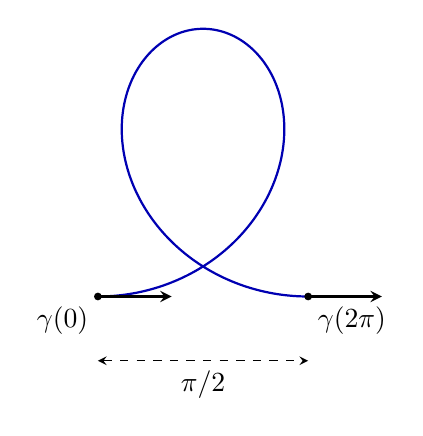
\begin{tikzpicture}[x=1.7cm,y=1.7cm,>=stealth]
	\draw[blue!70!black,thick,domain=0:360,samples=161,smooth,variable=\t] plot ({sin(\t)+0.5*(\t*pi/360+sin(2*\t)/4)},{1-cos(\t)+0.25*sin(\t)^2});
	\fill (0,0) circle (1.4pt) node[below left] {\(\gamma(0)\)};
	\fill ({pi/2},0) circle (1.4pt) node[below right] {\(\gamma(2\pi)\)};
	\draw[->,thick] (0,0)--(0.55,0);
	\draw[->,thick] ({pi/2},0)--({pi/2+0.55},0);
	\draw[<->,dashed] (0,-0.48)--node[below] {\(\pi/2\)} ({pi/2},-0.48);
\end{tikzpicture}

	\caption[切向量接合与位置闭合]{切向量接合与位置闭合。\(\varepsilon=\tfrac12\) 时，曲线转角从 \(0\) 增至 \(2\pi\)，两端的切向量相同，但端点相差 \((\pi/2,0)\)。箭头只表示相应端点的切向方向。}
	\label{g1:fig:closure-displacement}
\end{figure}

正面的例子是 \(k(s)=1/R\)、\(L=2\pi R\)，取初始切向量为 \((1,0)\)，积分得到
\[
	\gamma(s)=\bigl(R\sin(s/R),R(1-\cos(s/R))\bigr).
\]
三项闭合条件都成立，曲线恰为圆。若改用周期 \(4\pi R\)，同一公式仍满足条件，却把圆走了两遍。简单性还要求一个周期内只经过每个点一次。
